% !TeX root = supressed-anger.tex

\chapter{Algorithms}
\label{ch:algorithms}

\section{Fundamentals of Classification}

Classification, which is the task of assigning objects to one of several predefined categories, is a pervasive problem that encompasses many diverse applications \cite{pang2006introduction}.

\begin{figure}[!htp]
  \center
  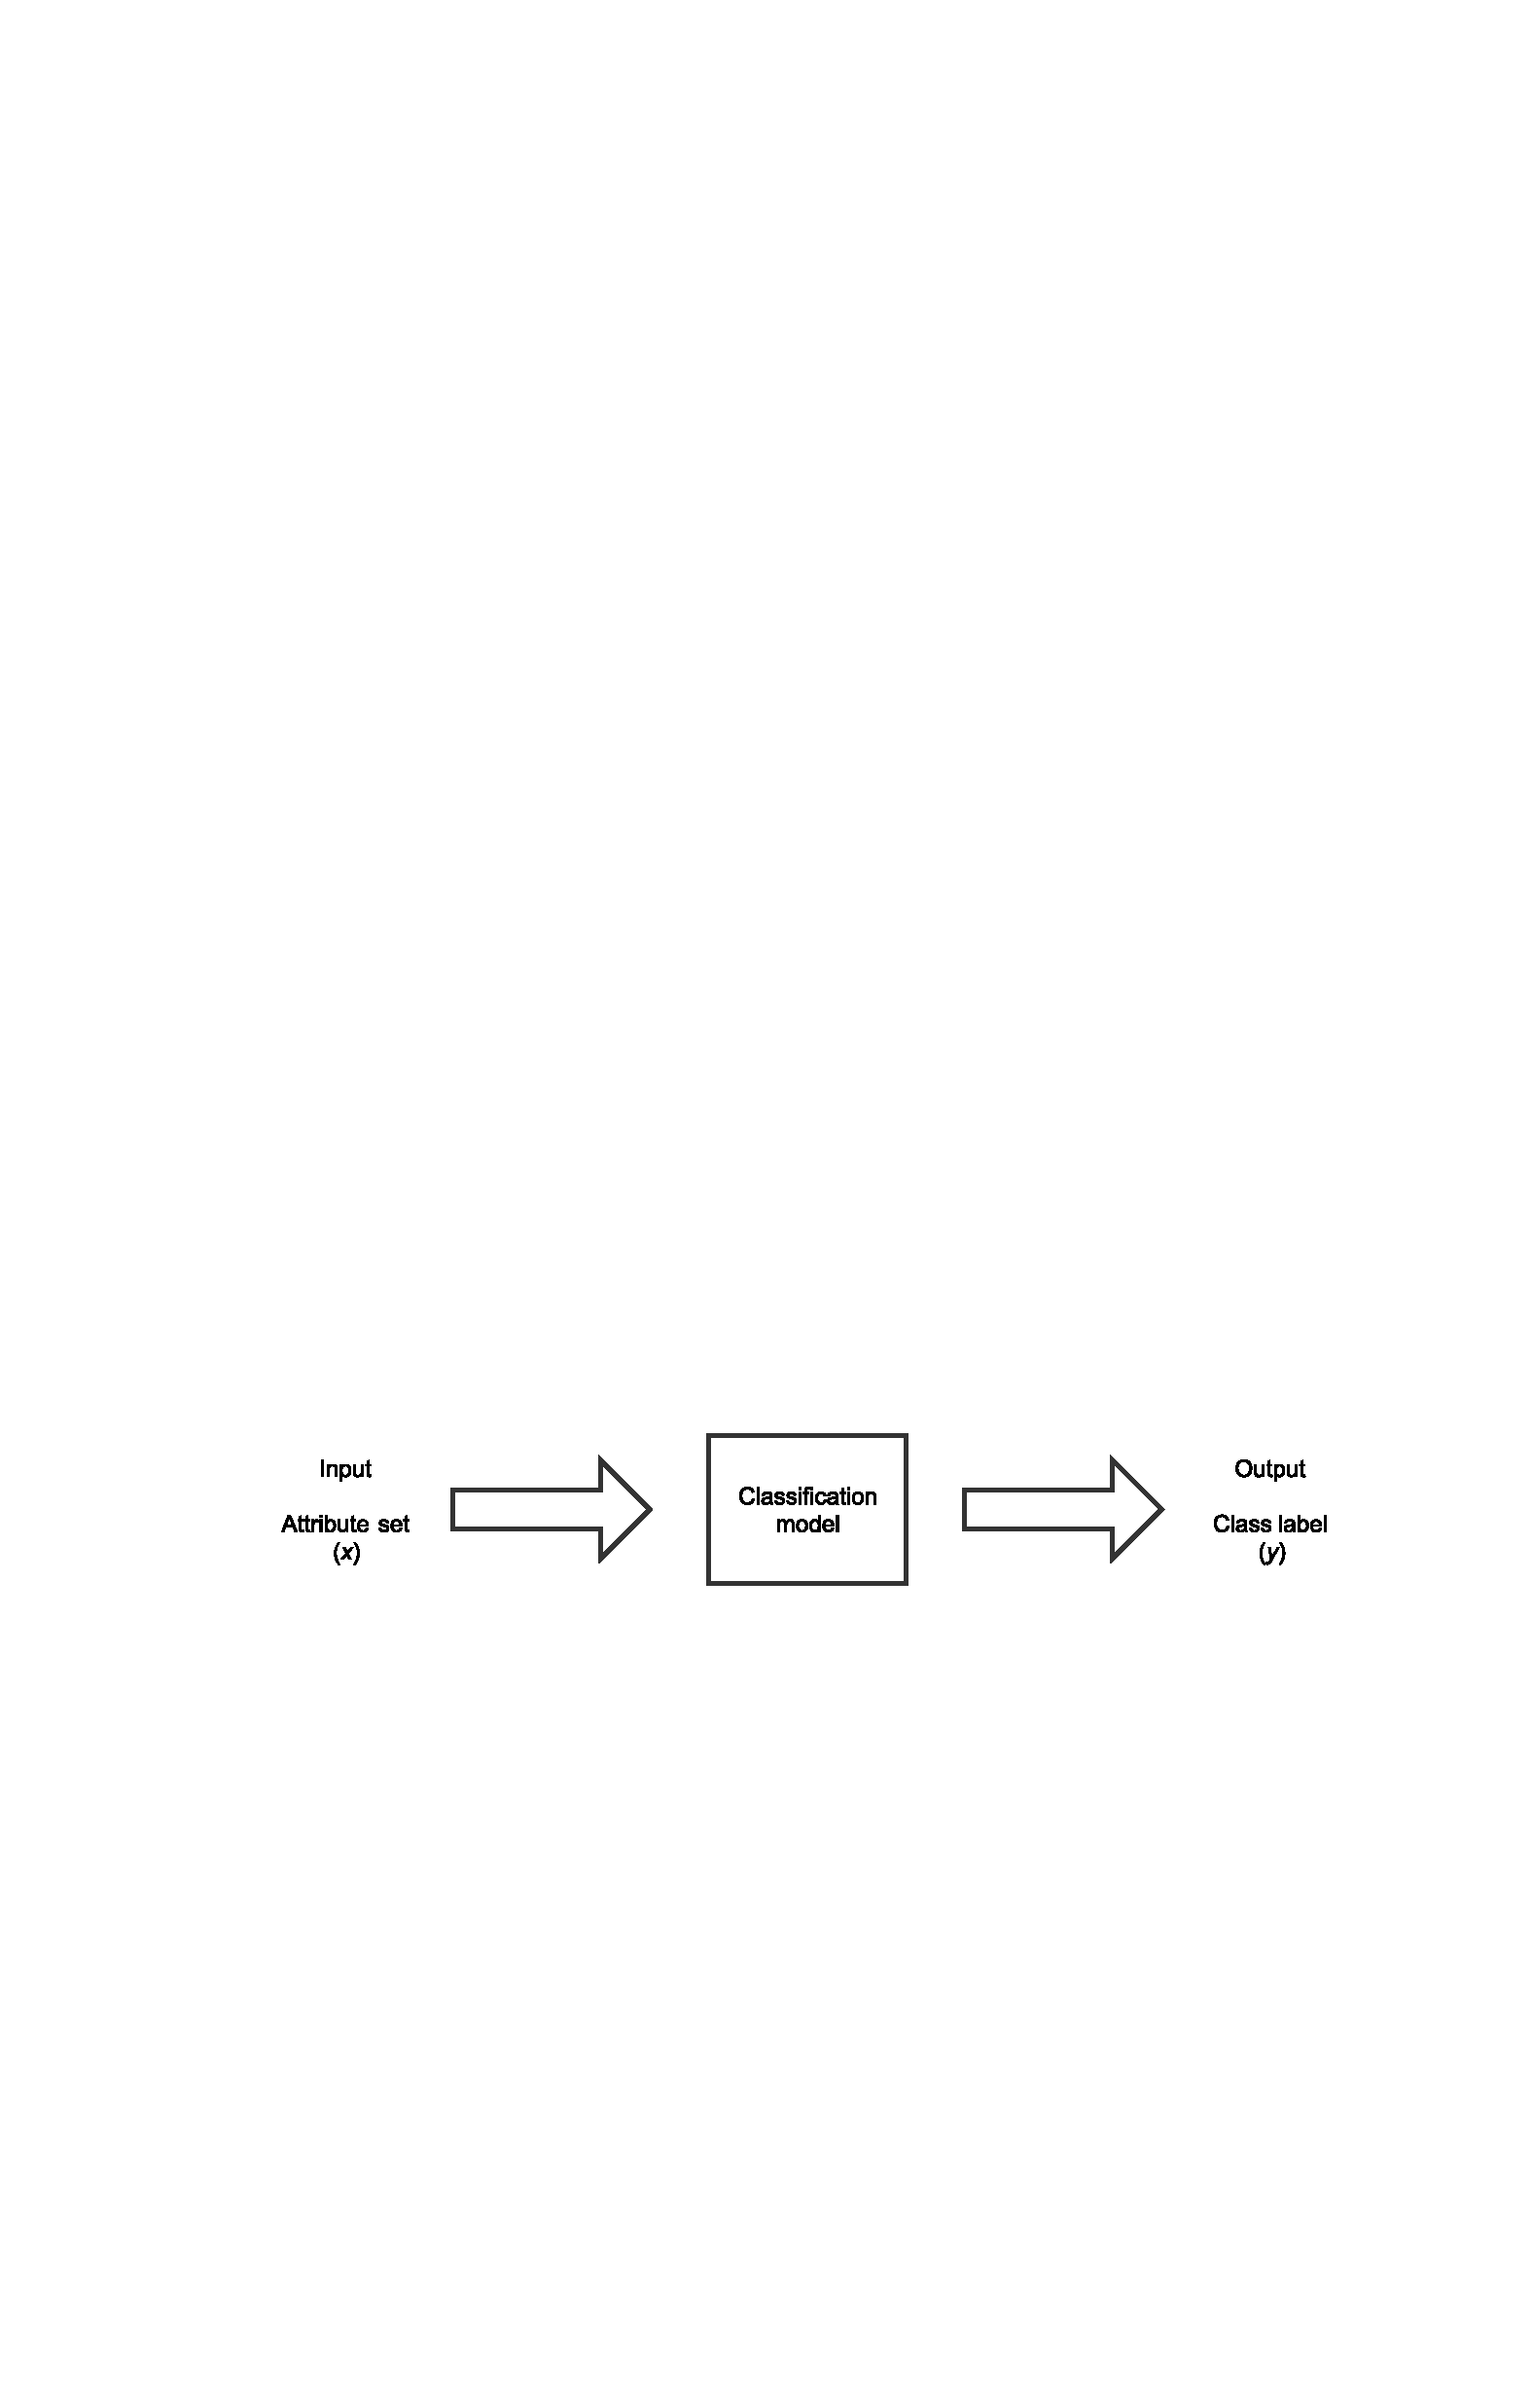
\includegraphics[width=\textwidth]{figures/classification}
  \caption{Classification as a task of mapping a set attributes $x$ into its fitting class label $y$.}
  \label{fig:classification_task}
\end{figure}

\FloatBarrier

The input data for a classification task is a collection of records. Each record, also known as an instance or example, is characterized by a tuple (x, y), where x is the attribute set and y is a special attribute, designated as the class label (also known as category or target attribute). Table 4.1 shows a sample data set used for classifying vertebrates into one of the following categories: mammal, bird, fish, reptile, or amphibian. The attribute set includes properties of a vertebrate such as its body temperature, skin cover, method of reproduction, ability to fly, and ability to live in water. Although the attributes presented in Table 4.1 are mostly discrete, the attribute set can also contain continuous features. The class label, on the other hand, must be a discrete attribute. This is a key characteristic that distinguishes classification from regression, a predictive modeling task in which y is a continuous attribute. Regression techniques are covered in Appendix D.

Definition (Classification). Classification is the task of learning a target function f that maps each attribute set x to one of the predefined class labels y.

The target function is also known informally as a classification model.

A classification model is useful for the following purposes.
Descriptive Modeling A classification model can serve as an explanatory tool to distinguish between objects of different classes.

Predictive Modeling A classification model can also be used to predict the class label of unknown records. As shown in Figure \ref{fig:classification_task}, a classification model can be treated as a black box that automatically assigns a class label when presented with the attribute set of an unknown record.

Classification techniques are most suited for predicting or describing data sets with binary or nominal categories. They are less effective for ordinal categories, because they do not consider the implicit order among the categories. Other forms of relationships, such as the subclass–superclass relationships among categories.

\section{Support Vector Machine}

There are four main advantages: Firstly it has a regularisation parameter, which makes the user think about avoiding over-fitting. Secondly it uses the kernel trick, so you can build in expert knowledge about the problem via engineering the kernel. Thirdly an SVM is defined by a convex optimisation problem (no local minima) for which there are efficient methods (e.g. SMO). Lastly, it is an approximation to a bound on the test error rate, and there is a substantial body of theory behind it which suggests it should be a good idea.
The disadvantages are that the theory only really covers the determination of the parameters for a given value of the regularisation and kernel parameters and choice of kernel. In a way the SVM moves the problem of over-fitting from optimising the parameters to model selection. Sadly kernel models can be quite sensitive to over-fitting the model selection criterion \cite{cawley2010over}

--------------------

SVMs are a new promising non-linear, non-parametric classification tech- nique, which already showed good results in the medical diagnostics, optical character recognition, elec- tric load forecasting and other fields.

Suitable for binary classification tasks.

The advantages of the SVM technique can be summarised as follows \cite{auria2008support}:

\begin{enumerate}
\item By introducing the kernel, SVMs gain flexibility in the choice of the form of the threshold separating solvent from insolvent companies, which needs not be linear and even needs not have the same func- tional form for all data, since its function is non-parametric and operates locally. As a consequence they can work with financial ratios, which show a non-monotone relation to the score and to the probability of default, or which are non-linearly dependent, and this without needing any specific work on each non-monotone variable.
\item Since the kernel implicitly contains a non-linear transformation, no assumptions about the functional form of the transformation, which makes data linearly separable, is necessary. The transformation oc- curs implicitly on a robust theoretical basis and human expertise judgement beforehand is not needed.
\item SVMs provide a good out-of-sample generalization, if the parameters C and r (in the case of a Gaussian kernel) are appropriately chosen. This means that, by choosing an appropriate generalization grade, SVMs can be robust, even when the training sample has some bias
\item SVMs deliver a unique solution, since the optimality problem is convex. This is an advantage compared to Neural Networks, which have multiple solutions associated with local minima and for this reason may not be robust over different samples.
\item With the choice of an appropriate kernel, such as the Gaussian kernel, one can put more stress on the similarity between companies, because the more similar the financial structure of two companies is, the higher is the value of the kernel. Thus when classifying a new company, the values of its financial ratios are compared with the ones of the support vectors of the training sample which are more similar to this new company. This company is then classified according to with which group it has the greatest similarity.
\end{enumerate}

--------------------------

Furthermore, $K(\bm{x}i, \bm{x}j ) \equiv \phi(\bm{x}_i)^T \phi(\bm{x}_j)$ is called the kernel function.

four basic kernels \cite{hsu2003practical}:

\begin{itemize}
\item \textbf{Linear:} $K(\bm{x}_i,\bm{x}_j) = \bm{x}^T_i \bm{x}_j$.
\item \textbf{Polynomial:} $K(\bm{x}_i,\bm{x}_j) = (\gamma \bm{x}^T_i \bm{x}_j + r)^d, \gamma > 0$.
\item \textbf{Radial Basis Function (RBF):} $K(\bm{x}_i,\bm{x}_j) = \exp(−\gamma \lVert \bm{x}_i − \bm{x}_j \rVert ^2),\gamma > 0$.
\item \textbf{Sigmoid:} $K(\bm{x}_i,\bm{x}_j) = \tanh(\gamma \bm{x}^T_i\bm{x}_j + r)$.
\end{itemize}

Here, $\gamma$, $r$, and $d$ are kernel parameters.

--------------------------

Support vector machines (SVM) were originally designed for binary classification \cite{hsu2002comparison}.

solving multi-class SVM in one step: “all-together” methods: [25], [27] and [7]. We then compare their performance with three methods based on binary classifications: “one-against-all,” “one-against-one,” and DAGSVM [23]. Our experiments indicate that the “one-against-one” and DAG methods are more suitable for practical use than the other methods. 

\section{K-Nearest Neighbor}

\section{Neural Networks}
